
%(BEGIN_QUESTION)
% Copyright 2015, Tony R. Kuphaldt, released under the Creative Commons Attribution License (v 1.0)
% This means you may do almost anything with this work of mine, so long as you give me proper credit

A current transformer with a ratio of 1000:5 senses line current in a system where the inductance-to-resistance ratio is 6-to-1.  The CT has a rating of C800, an internal winding resistance of 0.2 ohms, and is connected to a protective relay having a burden of 0.65 ohms (resistive) through 12 gauge copper wire.  Sketch an equivalent schematic diagram of this circuit, and calculate the maximum cable length connecting this CT to the relay so that it does not become excessively burdened with a symmetrical fault current of 3.8 kA.

\vfil 

\underbar{file i02608}
\eject
%(END_QUESTION)





%(BEGIN_ANSWER)

This is a graded question -- no answers or hints given!

%(END_ANSWER)





%(BEGIN_NOTES)

First, the equivalent schematic diagram:

$$\includegraphics[width=15.5cm]{i02608x01.eps}$$

The CT's C800 rating and 0.2 ohm internal winding resistance tells us it is capable of generating 820 volts at the winding (based on the rating's assumption of 100 $\times$ full-load current while providing 800 volts at the CT connection terminals) with no DC components present.  Since this system has an $X \over R$ ratio of 6, we must de-rate this 820 volt theoretical maximum value to account for the presence of DC which will predispose the CT's core to magnetic saturation:

$$V_W = {V_{max} \over {1 + {X \over R}}} = {820 \hbox{ V} \over {1 + 6}} = 117.1 \hbox{ V}$$

We need to determine the maximum amount of cable resistance permissible for this CT to deliver stepped-down fault current to the relay without demanding more than 117.1 volts at its winding.

\vskip 10pt

Calculating fault current:

$$I_{CT} = \left({3800 \hbox{ A} \over 1} \right) \left({5 \over 1000} \right) = 19.00 \hbox{ A}$$

Using Ohm's Law to calculate maximum total circuit resistance:

$$R_{total} = {V \over I} = {117.1 \hbox{ V} \over 19.00 \hbox{ A}} = 6.165 \> \Omega$$

Subtracting the relay and CT winding resistances from this total figure will give the cable resistance:

$$R_{total} = R_{CT} + R_{relay} + R_{cable}$$

$$R_{cable} = R_{total} - (R_{CT} + R_{relay})$$

$$R_{cable} = 6.165 \> \Omega - (0.2 \> \Omega + 0.65 \> \Omega) = 5.315 \> \Omega$$

The resistance of 12 gauge copper wire is given by the following calculation:

$$R_{wire} = {e^{(12)(0.232) - 2.32}} \> \Omega \hbox{ per 1000 ft}$$

$$R_{wire} = 1.59 \> \Omega \hbox{ per 1000 ft}$$

\filbreak

Total wire length may be calculated by dividing the total wire resistance by the resistance per 1000 feet, or multiplying total wire resistance by 1000 feet over 1.59 $\Omega$:

$$\left({5.315 \> \Omega \over 1}\right) \left({1000 \hbox{ ft} \over 1.59 \> \Omega}\right) = 3342.1 \hbox{ ft}$$

This figure of 3342.1 feet is total conductor length.  The cable, possessing two conductors, will be half as long, or {\bf 1671.1 feet}.

%INDEX% Electronics review: current transformer (CT)
%INDEX% Protective relay: CT circuit wire resistance

%(END_NOTES)


